The purpose of study III is to evaluate the implemented telehealth system in a real context. We here bring details on methods used.

\textbf{Preliminary Data Collection}

We collected preliminary data prior to the study of two reasons, one being the system's dashboard only function when having two measures to compare in order to show upward or downward trends, the other was for the participants to have data to reflect on from the start of the trial, which we found important because of the relatively short trial period. The template used to collect the preliminary data can be seen on attached CD. The dates in the template varied depending on when a patient was enrolled in the study.

\textbf{Diary}

During the trial period, the patients were asked to write in a diary after each use. To provide inspiration on what to report on in the diary, we taped questions on the first page of the diary. The questions were:
\begin{itemize}
	\item What did you think while using the system? (e.g. on page for entering data, page showing previous measures, page for overview and the system's question)
	\item What in the system generated thoughts?
	\item How was the experience of using the system?
	\item What puzzled you in the system?
	\item What did you learn from using the system?
	\item How has the system helped you?
	\item Suggestions for improvements.
\end{itemize}
When patients were given the diary before starting using the system, the patients were told that the questions only functioned as inspiration and it was not required to write, only if they had something on mind.

\textbf{Activity Plan}

Demographic questions (from the questionnaire) and the questions from the interview are both listed in the Activity Plan, which is attached as appendix, \ref{ap3}.

\textit{Demographics}

Demographic data of each patient completing the study can be found on attached CD (in Final Evaluation.xlsx).

\textit{Interview}

The interview was conducted as a semi-structured interview with focus on typical COPD-activities such as use of pulse oximeter, medication use etc. We searched for a change in COPD-activities during the use of the system. When a change was identified we drilled further down, asking why it was changed to see if it related to the system use. If it related to the system use we again drilled further down to find possible features in the user interface that fostered reflection and provided a change in perspective and activity. All the interviews were audio-recorded. The recordings can be found on detached CD.

\textit{Cue recall}

To cue recall from using the system during the interview, we made two initiatives. First, we prepared screen-shots of patients' dashboards showing events of interest (e.g. worsening or improvement in measures between two days). We here bring an example of the two screen-shots that was prepared for P4. 

\begin{figure}[h]
  \centering
  \begin{minipage}[b]{0.45\textwidth}
    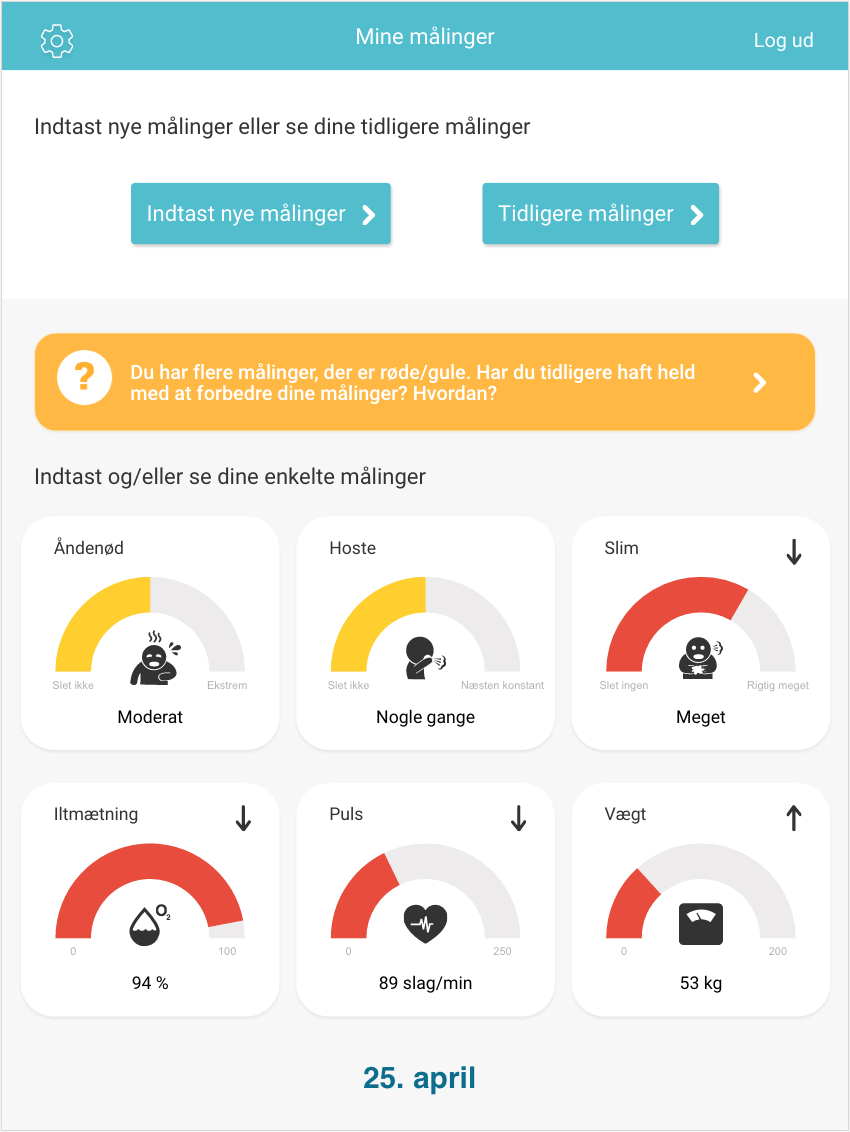
\includegraphics[width=\textwidth]{images/study3/Gunnar12.png}
    \caption{Shows status from first day of use (April 25) for P4.}
    \label{fig:gunnar12}
  \end{minipage}
  \hfill
  \begin{minipage}[b]{0.45\textwidth}
    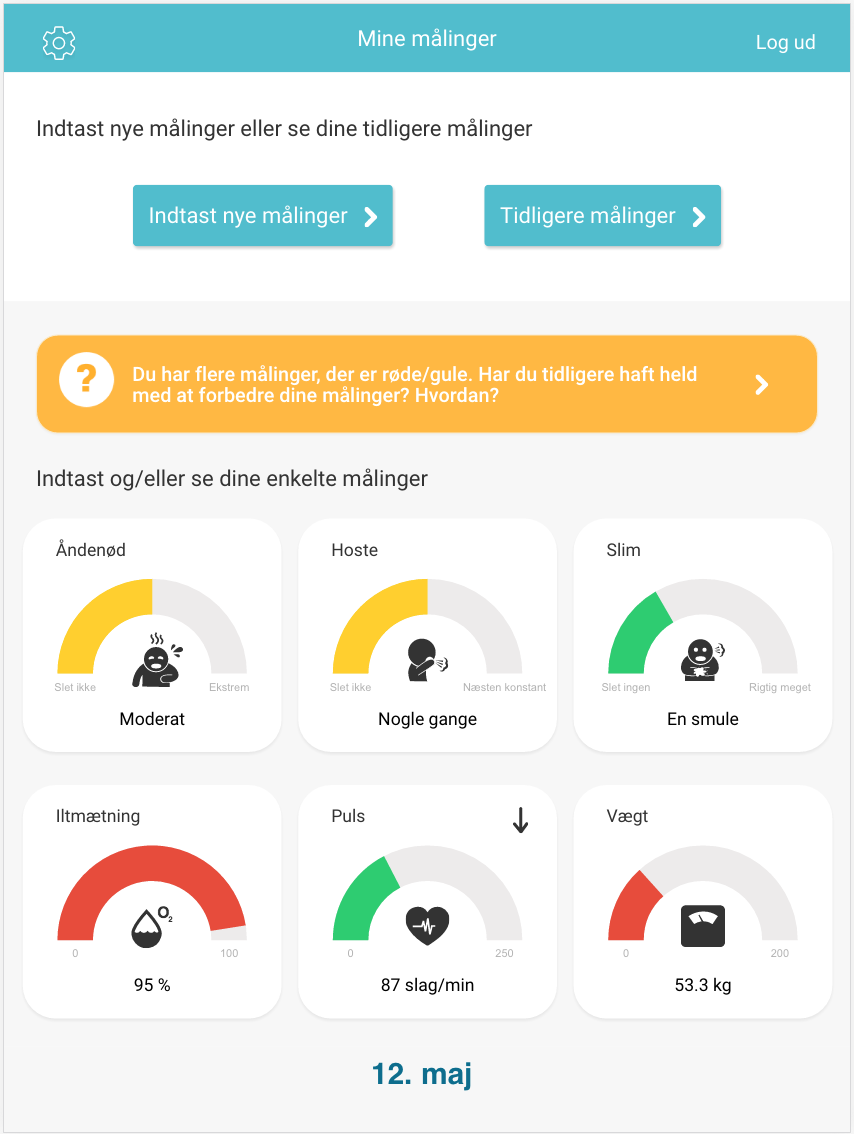
\includegraphics[width=\textwidth]{images/study3/Gunnar22.png}
    \caption{Shows status from last day of use (May 12) for P4 before evaluation.}
    \label{fig:gunnar22}
  \end{minipage}
\end{figure}

Above pictures show an improvement in health status. We hoped it could help replaying the situation between the two days and reveal the reflection that potentially occurred and the feelings related to the development.
All the prepared screen-shots can be found on attached CD.

Our second initiative in the effort of cueing recall was to get an overview of each patients' use of the system by going through the system log and find situation where reflection potentially could have occurred. For instance we looked for an outlier in measures, what reflective questions each patient had received and what the patient turned to when the reflective question pointed at a design feature. The overview also included basic information as number of entries, what pages the user had visited and what features the patient had used. This overview is also included on the detached CD (called Overview.pdf). The system log can also be found on the CD (in Final Evaluation.xlsx).


\textbf{Data processing}

We transcribed the interviews from the audio recordings and coded the interviews. This data is included on attached CD (in Final Evaluation.xlsx).
